\chapter{Preliminaries}
\label{ch:prelims}

Here we explain the basic definitions as well as the notation used in the following chapters.

\section{Probability Theory and Inequalities}

We say an event $E(n)$ over a sample space $\Omega$
happens with high probability (w.h.p.) when
\begin{equation}
    \lim_{n\to\infty}{\Pr_\Omega[E(n)]}=1
\end{equation}

\subsection{Union Bound}

If $\Omega$ is a sample space and $E_1,\ldots,E_n$ are events over $\Omega$, then
\begin{equation}
    \Pr_\Omega\left[\bigcup_{i=1}^n{E_i}\right]\leq\sum_{i=1}^m{\Pr_\Omega\left[E_i\right]}
\end{equation}

\subsection{Chernoff Bounds}

% https://en.wikipedia.org/wiki/Chernoff_bound#Multiplicative_form_(relative_error)
Let $X_1,\ldots,X_n\in\{0,1\}$ be independent random variables,
and $X=\sum_{i=1}^n{X_i}$ with expected value
$\mu=\E[X]=\sum_{i=1}^n{\Pr[X_i=1]}$.
\begin{align}
    %\Pr[X\geq a]=\Pr[e^{tX}&\geq e^{ta}]\leq\frac{\E[e^{tX}]}{e^{ta}},\text{ for }t>0\\
    \Pr[X\geq(1+\delta)\mu]&\leq
    \begin{cases}
        \exp(-\delta^2\mu/(2+\delta)) & \quad \text{if } \delta>1,\\
        \exp(-\delta^2\mu/3) & \quad \text{if } 0<\delta\leq 1.
    \end{cases}\\
    \label{eq:chernoff-lower-tail}
    \Pr[X\leq(1-\delta)\mu]&\leq \exp(-\delta^2\mu/2),\text{ for }0<\delta<1
\end{align}
We can combine these two:
\begin{equation}
    \label{eq:chernoff-combined}
    \Pr[|X-\mu|\geq\delta\mu]\leq 2\;\exp(-\delta^2\mu/3),\text{ for }0<\delta<1
\end{equation}

\subsection{Combinations}

\begin{equation}
    \left(\frac{n}{k}\right)^k
    \leq\binom{n}{k}=\frac{n!}{k!(n-k)!}
    \leq\left(\frac{en}{k}\right)^k
\end{equation}

It is easy to show:

$\frac{n}{k}\leq\frac{n-m}{k-m}$, for $0\leq m<k\leq n$,
so $\left(\frac{n}{k}\right)^k=\frac{n}{k}\ldots\frac{n}{k}$
$\leq\frac{n}{k}\frac{n-1}{k-1}\ldots\frac{n-k+1}{1}=\binom{n}{k}$

$\binom{n}{k}=\frac{n}{k}\frac{n-1}{k-1}\ldots\frac{n-k+1}{1}
\leq\frac{n^k}{k!}=\frac{k^k}{k!}\left(\frac{n}{k}\right)^k\leq\left(\frac{en}{k}\right)^k$

The last step uses the Maclaurin series of the exponential function:
\begin{equation}
    e^k=\sum_{n=0}^{\infty}{\frac{k^n}{n!}}\geq\frac{k^k}{k!}
\end{equation}

\subsection{Stirling's Approximation and the Number of Perfect Matchings}

Let $M(m)$ denote the number of perfect matchings on the set of even size $m$:
\begin{equation}
    M(m)=(m-1)!!=(m-1)(m-3)\ldots(3)(1)=\frac{m!}{2^{m/2}(m/2)!}
\end{equation}

We can use Stirling's approximation:
\begin{equation}
    \label{eq:stirling-approx}
    m!=(1+o(1))\sqrt{2\pi m}(m/e)^m
\end{equation}
\begin{equation}
    \label{eq:number-of-matchings}
    M(m)=(1+o(1))\frac{\sqrt{2\pi m}(m/e)^m}{2^{m/2}\sqrt{\pi m}(m/2e)^{m/2}}
    =(1+o(1))\sqrt{2}(m/e)^{m/2}
\end{equation}

\subsection{The Upper Bounds for the Sum of a Special Series}

The following sum $S_n$ occurs in several proofs. We will need to upper bound it
for $n\to\infty$ and some constants $0<\alpha\leq 1/2$, $c_1>0$, and $c_2>0$:
\begin{equation}
    S_n=\sum_{s=1}^{\alpha n}{\left(c_1(s/n)^{c_2}\right)^s}
\end{equation}
Each subsequent bound will require more rigorous analysis.

\begin{proposition}
    $S_n<1$, when $c_2\geq1+\log c_1$.
\end{proposition}

\begin{proof}
    $S_n=\sum_{s=1}^{\alpha n}{\left(c_1(s/n)^{c_2}\right)^s}
    \leq\sum_{s=1}^{\alpha n}{\left(c_1\alpha^{c_2}\right)^s}
    \leq\sum_{s=1}^{\infty}{2^{-c_3s}}
    \leq\sum_{s=1}^{\infty}{2^{-s}}<1$,
    where $c_3=c_2-\log c_1$ is a constant greater or equal $1$:
    \begin{gather}
        c_3\geq 1\iff c_2\geq 1+\log c_1\\
        c_1\alpha^{c_2}\leq c_1 2^{-c_2}=2^{-c_3}\leq 2^{-1}
    \end{gather}
\end{proof}

\begin{proposition}
    \label{pro:bound-prob-small-sets}
    $S_n\leq o(1)$ for some sufficiently small $\alpha$.
\end{proposition}

\begin{proof}
    First, we pick $\alpha$ so that $\left(c_1\alpha^{c_2}\right)<1/10$,
    using some constant $c_3>10$:
    \begin{equation}
        \alpha=(c_1c_3)^{-1/c_2}
    \end{equation}
    
    Then we consider small and large values of $s$ separately.
    Define $0<\epsilon<1$ such that
    \begin{gather}
        \epsilon<(1-\epsilon)c_2\iff\epsilon<\frac{c_2}{1+c_2}\\
        S'=\sum_{s=1}^{n^\epsilon}{\left(c_1(s/n)^{c_2}\right)^s}
        \leq\sum_{s=1}^{n^\epsilon}{\left(\frac{c_1}{n^{(1-\epsilon)c_2}}\right)^s}
        \leq n^\epsilon\frac{c_1}{n^{(1-\epsilon)c_2}}=o(1)\\
        S''=\sum_{s=n^\epsilon+1}^{\alpha n}{(c_1(s/n)^{c_2})^s}
        <\sum_{s=n^\epsilon+1}^{\alpha n}{10^{-s}}
        \leq\frac{\alpha n}{10^{n^\epsilon}}=o(1)
    \end{gather}
    
    $S_n=S'+S''\leq o(1)$.
\end{proof}

\begin{proposition}
    \label{pro:bound-prob-large-sets}
    $S_n\leq o(1)$ for any $\alpha\leq 1/2$ and $c_2>\max\{1,\log c_1\}$.
    
    Moreover, $c_1$ and $c_2$ can be superconstants in terms of $n$,
    as long as $c_1=o\left(n^{c_2-1}\right)$.
\end{proposition}

\begin{proof}
    The argument is identical to the known one~\cite{gms03}.
    
    For $s\geq1$, let's define $f(s)=\left(c_1(s/n)^{c_2}\right)^s$, then
    $S_n=\sum_{s=1}^{\alpha n}{f(s)}$.
    The first two derivatives will help us understand the behavior of $f(s)$.
    
    First, the simple case is when $c_1=c_2=1$:
    \begin{gather*}
        \frac{d}{ds}\left(\frac{s}{n}\right)^s
        =\frac{d}{ds}\exp\left(s\,\ln\frac{s}{n}\right)
        =\left(\frac{s}{n}\right)^s\left(\ln\frac{s}{n}+s\frac{1/n}{s/n}\right)
        =\left(\frac{s}{n}\right)^s\left(\ln\frac{s}{n}+1\right)\\
        \frac{d^2}{ds^2}\left(\frac{s}{n}\right)^s
        =\left(\frac{s}{n}\right)^s\left(\frac{1}{s}+\left(1+\ln\frac{s}{n}\right)^2\right)>0
    \end{gather*}
    We can see that $\left(\frac{s}{n}\right)^s$ is concave up for any $s\geq1$
    and attains its minimum at $s=n/e$.
    
    Then we perform similar steps for $f(s)$:
    \begin{equation}
        \begin{split}
            f'(s)=&\frac{d}{ds}\left(c_1\left(\frac{s}{n}\right)^{c_2}\right)^s
            =\frac{d}{ds}\exp\left(
                s\,
                \ln\left(c_1\left(\frac{s}{n}\right)^{c_2}\right)
            \right)=\\
            =&f(s)\left(
                \ln\left(c_1\left(\frac{s}{n}\right)^{c_2}\right)
                +s\frac{c_1c_2(s/n)^{c_2-1}(1/n)}{c_1(s/n)^{c_2}}
            \right)=\\
            =&f(s)\left(\ln\left(c_1\left(\frac{s}{n}\right)^{c_2}\right)+c_2\right)=\\
            =&f(s)c_2\left(\ln\frac{c_1^{1/c_2}s}{n}+1\right)=\\
            =&f(s)c_2\left(\ln\frac{s}{n}+\frac{\ln c_1}{c_2}+1\right)
        \end{split}
    \end{equation}
    \begin{equation}
        \begin{split}
            f''(s)=&\frac{d^2}{ds^2}\left(\frac{s}{n}\right)^s
            =\left(\frac{s}{n}\right)^s\left(\frac{1}{s}+\left(1+\ln\frac{s}{n}\right)^2\right)=\\
            % (3*((x/y)^7))^x * (log(3*((x/y)^7))+7)
            =&\frac{c_2}{s}f(s)+c_2\left(\ln\frac{s}{n}+1\right)f'(s)+(\ln c_1)f'(s)=\\
            =&\frac{c_2}{s}f(s)+c_2\left(\ln\frac{s}{n}+\frac{\ln c_1}{c_2}+1\right)f'(s)=\\
            =&\frac{c_2}{s}f(s)+\frac{(f'(s))^2}{f(s)}
        \end{split}
    \end{equation}
    
    Define $s_0$ to be an extreme point of $f(s)$:
    \begin{gather}
        f'(s_0)=0\\
        \ln\frac{c_1^{1/c_2}s}{n}=-1\\
        s_0=\frac{n}{ec_1^{1/c_2}}
    \end{gather}
    
    And verify that $f''(s)>0$ for any $s\geq1$:
    \begin{gather}
        \frac{c_2}{s}f(s)+\frac{(f'(s))^2}{f(s)}>0\\
        \frac{c_2}{s}+\left(\frac{f'(s)}{f(s)}\right)^2>0
    \end{gather}
    
    \begin{gather}
        \begin{cases}
            f'(s)<0 & \quad \text{if } s<s_0,\\
            f'(s)=0 & \quad \text{if } s=s_0,\\
            f'(s)>0 & \quad \text{if } s>s_0.
        \end{cases}\\
        f''(s)>0,\text{ for }s\in[1;\alpha n]
    \end{gather}
    
    Therefore, $f(s)$ is concave up on the whole interval
    $[1;\alpha n]$ with these endpoints:
    \begin{gather}
        f(1)=\frac{c_1}{n^{c_2}}\\
        f(\alpha n)=\left(c_1\alpha^{c_2}\right)^{\alpha n}
        \leq\left(c_1 2^{-c_2}\right)^{\alpha n}
    \end{gather}
    
    $f(1)=o(1/n)$ when $c_2>1$, and $f(\alpha n)=o(1/n)$
    when $c_1 2^{-c_2}<1\iff c_2>\log c_1$.
    
    Additionally, both $c_1$ and $c_2$ might be superconstants in terms of $n$,
    if this holds:
    \begin{equation}
        c_1=o\left(n^{c_2-1}\right)
    \end{equation}

    To sum up, given $c_2>\max\{1,\log c_1\}$,
    
    $S_n=\sum_{s=1}^{\alpha n}{f(s)}
    \leq\sum_{s=1}^{\alpha n}{\max\{f(1),f(\alpha n)\}}
    =o\left(\frac{\alpha n}{n}\right)=o(1)$.
\end{proof}

Note that if $c_2$ in~\autoref{pro:bound-prob-large-sets} is not large enough,
there is no advantage in terms of the size of expanding sets
compared to~\autoref{pro:bound-prob-small-sets}:
\begin{equation}
    c_1\alpha^{c_2}<1\iff\alpha<c_1^{-1/c_2}
\end{equation}

\section[Generalized Harmonic Numbers and Riemann Zeta Function]
        {Generalized Harmonic Numbers and Riemann Zeta\\Function}

Generalized harmonic numbers are defined as
\begin{equation}
    H_{n,m}=\sum_{k=1}^{n}\frac{1}{k^m}
\end{equation}

We will extensively use these approximations for large $n$:
\begin{equation}
    H_{n,\beta}\approx
    \begin{cases}
        \frac{n^{1-\beta}}{1-\beta} & \quad \text{if } \beta<1,\\
        \ln n & \quad \text{if } \beta=1,\\
        \zeta(\beta) & \quad \text{if } \beta>1.
    \end{cases}
\end{equation}

The zeta function was introduced in 1737 by Euler, later Riemann allowed its argument to be a complex number.
\textit{Riemann zeta function} is defined for all $s\in\mathbb{C}$ with $\Re(s)>1$, see~\autoref{fig:zeta}:
\begin{equation}
    \label{eq:riemann-zeta-function}
    \zeta(s)=\sum_{n=1}^{\infty}\frac{1}{n^s}
\end{equation}
% https://math.stackexchange.com/q/876166
For $x\in\mathbb{R}$, we know that $\zeta(x)\approx 1+2^{-x}$ when $x\gg 1$,
and $\lim_{x\to\infty}\zeta(x)=1$.

For $m>1$ as $n\to\infty$, applying the Euler-Maclaurin formula~\eqref{eq:euler-maclaurin-formula}
to the remainders $\sum_{n>N}{n^{-s}}$ of the sum~\eqref{eq:riemann-zeta-function}
provides the following connection:
\begin{gather}
    \zeta(s)=H_{N,s}+\frac{1}{(s-1)N^{s-1}}+\frac{1}{2N^s}+O\left(\frac{1}{N^{s+1}}\right),\quad\text{ for some }N\gg1\\
    H_{n,m}=\zeta(m)-\frac{1}{(m-1)n^{m-1}}-\frac{1}{2n^m}-O\left(\frac{1}{n^{m+1}}\right)
    =\zeta(m)-o(1)
\end{gather}

\begin{figure}
    \centering
    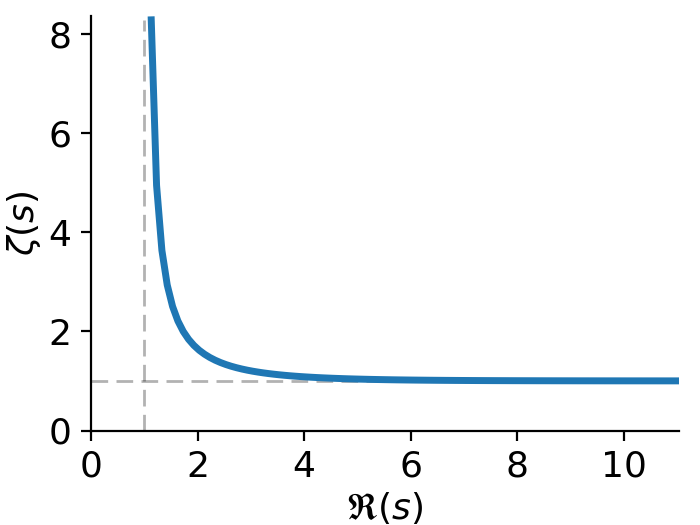
\includegraphics[scale=0.75]{images/generated/zeta}
    \caption[Riemann zeta function]{Riemann zeta function for $s\in\mathbb{C}$ with $\Re(s)>1$ and $\Im(s)=0$}
    \label{fig:zeta}
\end{figure}

\section{Gilbert and \texorpdfstring{Erd\H{o}s-R\'enyi}{Erdos-Renyi} Random Graphs}

The most commonly used models of uniform random graphs are $G(n,p)$ and $G(n,m)$
introduced by Gilbert~\cite{gil59} and by Erd\H{o}s and R\'enyi~\cite{er59}.

$G(n,p)$ contains all graphs where each pair of vertices
is connected by an edge with probability $p$.
We denote the maximum number of edges $N=\binom{n}{2}$,
then the expected number of edges in such graphs is $pN$.
\begin{gather}
    \Pr_{G\sim G(n,p)}[G\text{ has }m\text{ edges}]=\binom{N}{m}p^m(1-p)^{N-m}\\
    \Pr_{G\sim G(n,p)}[\deg(v)=k]=\binom{n-1}{k}p^k(1-p)^{n-k-1},\text{ for }v\in V(G)
\end{gather}

On the other hand, $G(n,m)$ describes the graphs with $n$ vertices and exactly $m$ edges.
They may be generated by successively selecting $m$ pairs of not yet connected vertices,
so that each of $\binom{N}{m}$ possible graphs is chosen uniformly at random.

Erd\H{o}s and R\'enyi~\cite{er60} depict the following structural properties of $G(n,p)$ graphs.
When $p=o(1/n)$, the graph is simply a disjoint union of trees.
Then consider the case $p=c/n$, where $c$ is some constant.
If $c<1$, the size of the largest component is just $O(\log n)$,
at the critical point $c=1$ its size is $\Theta\left(n^{2/3}\right)$,
and a unique giant component of size $\Theta(n)$ emerges when $c>1$.
Finally, the graphs are disconnected  w.h.p. when $p<(1-\epsilon)\log n/n$
and become connected w.h.p. when $p>(1+\epsilon)\log n/n$, for any $\epsilon>0$~\cite{er59}.

As per Chung and Lu~\cite{cl01,cl04}, the diameter of $G(n,p)$ is
$\Theta(\log n)$ when $p=c/n$, for some constant $c>1$,
and $(1+o(1))\frac{\log n}{\log np}$ if $p=\omega(1/n)$.
The diameter of a disconnected graph is assumed to be the maximum
diameter of its connected components.

%If $np\geq c>1$ for some constant $c$,
%and $\lim_{n\to\infty}{\frac{\log n}{\log np}}=\infty$,
%then the average distance of $G(n,p)$ is $(1+o(1))\frac{\log n}{\log np}$ w.h.p.~\cite{cl04}

If we choose $m=pN$, $G(n,p)$ and $G(n,m)$ models are almost identical for large $n$
and $p>\log n/n$, but some important properties might be different for smaller $p$.
For example, let $p=3/n$ and so $m=\frac{3}{2}(n-1)$.
In this case $G(n,p)$ is disconnected w.h.p., while $G(n,m)$ yields
a connected graph with high expansion~\cite{mah09} as almost 3-regular.

Independence of edges of $G(n,p)$ makes it similar to our coin toss model for power-law graphs,
and $G(n,m)$ corresponds more to $m$ edges model and permutation model,
which will be defined in~\autoref{ch:powerlaw}.

\section{Expander Graphs}

\subsection{Combinatorial Expansion}

First, we look at the combinatorial notions of expansion.

\begin{definition}
    A graph $G$ is called \textit{$(\alpha n,\gamma)$ edge expander} if for some $\gamma>0$
    \begin{equation}
        \min_{\substack{S\subset V\\0<|S|\leq\alpha n}}\frac{|\partial S|}{|S|}\geq\gamma,
    \end{equation}
    where the left-hand side expression with $\alpha=1/2$ is \textit{the Cheeger constant $h(G)$}, and
    \begin{equation}
        \partial S=e(S,V\backslash S)=\{(u,v)\in E\;|\;u\in S,v\in V\backslash S\}.
    \end{equation}
\end{definition}

\begin{definition}
    Analogously, \textit{$(\alpha n,\gamma)$ vertex expander} satisfies the following condition:
    \begin{equation}
        \min_{\substack{S\subset V\\0<|S|\leq\alpha n}}\frac{|N_G(S)|}{|S|}\geq\gamma,
    \end{equation}
    where $N_G(S)$ is the external neighborhood of $S$ in $G$, i.e.,
    \begin{equation}
        N_G(S)=\{v\in V\backslash S\;|\;\exists u\in S, (u,v)\in E\}.
    \end{equation}
\end{definition}

\begin{definition}
    \textit{$(\alpha n,\gamma)$ unique-neighbor expander} is a graph satisfying
    \begin{equation}
        \min_{\substack{S\subset V\\0<|S|\leq\alpha n}}
        \frac{|\{v\in V\backslash S\;|\;v\text{ is adjacent to exactly one }u\in S\}|}{|S|}\geq\gamma.
    \end{equation}
\end{definition}

\subsection{Spectral Expansion}

Let the vertex $v$ have $\deg(v)$ and define $T=diag(\deg(v))$.
The Laplacian of $G$ without loops or multiple edges is
$\Laplacian=T^{-\frac{1}{2}}LT^{-\frac{1}{2}}$.
If $G$ is \textit{d-regular}, then $\Laplacian=I-A/d$~\cite{chu97}.
\begin{align}
    L_{u,v}&=
    \begin{cases}
        \deg(v) & \quad \text{if } u=v \text{,}\\
        -1      & \quad \text{if } (u,v)\in E(G),\\
        0       & \quad \text{otherwise.}
    \end{cases}\\
    \Laplacian_{u,v}&=
    \begin{cases}
        1                                   & \quad \text{if } u=v \text{ and } \deg(v) \neq 0 \text{,}\\
        -\frac{1}{\sqrt{\deg(u)\deg(v)}}    & \quad \text{if } (u,v)\in E(G),\\
        0                                   & \quad \text{otherwise.}
    \end{cases}
\end{align}

The spectrum of $G$ are the eigenvalues of $\Laplacian$ $\{\lambda_1,\ldots,\lambda_n\}$,
$0=\lambda_1 \leq \lambda_2 \leq \dots \leq \lambda_{n}$.
Eigenvalue $0$ has eigenvector $T^{1/2}\mathbf{1}$.

Let $g:V\to\mathbb{R}$ be an arbitrary function, $g=T^{1/2}f$ for some $f$,
and both $g$ and $f$ are viewed as column vectors.
The Rayleigh quotient is
\begin{equation}
    \frac{\langle g,\Laplacian g \rangle}{\langle g,g \rangle}
    =\frac{\sum_{u \sim v}{(f(u)-f(v))^2}}{\sum_{v}{f(v)^2\deg(v)}}
\end{equation}
%    d1 0 -1        d1f1-f3                                        d1=1
% f, 0  d2 0 f = f, d2f2     = f1(d1f1-f3)+f2(d2f2)+f3(-f1+d3f3) = d2=0 = d1f1^2-f1f3+d2f2^2+d3f3^2-f1f3
%    -1 0 d3        -f1+d3f3                                       d3=1
%
% Laplacian*v=lambda*v=(0 0 ... 0)
% 1             0 -1/sqrt(d1d3)   sqrt(d1)   sqrt(d1)-1/sqrt(d1)   0
% 0             0 0             * sqrt(d2) = 0                   = 0
% -1/sqrt(d1d3) 0 1               sqrt(d3)   -1\sqrt(d3)+sqrt(d3)  0
and it is related to the spectral expansion of $G$, also known as the spectral gap,

\begin{equation}
    \lambda_G=\lambda_2=\inf_{f \perp T^{\frac{1}{2}}\mathbf{1}}
    \frac{\sum_{u \sim v}{(f(u)-f(v))^2}}{\sum_{v}{f(v)^2\deg(v)}}
\end{equation}

%\begin{equation}
%    Tr(M)=\sum_v{M_{v,v}}=\sum_i{\lambda_i}
%\end{equation}
%
%The Laplacian of a weighted $G$:
%\begin{align}
%    L&=
%    \begin{cases}
%        \deg(v)-w(v,v)  & \quad \text{if } u=v \text{,}\\
%        -w(u,v)         & \quad \text{if } (u,v)\in E(G),\\
%        0               & \quad \text{otherwise.}
%    \end{cases}\\
%    \Laplacian&=
%    \begin{cases}
%        1-\frac{w(u,v)}{\deg(v)}                & \quad \text{if } u=v \text{ and } \deg(v) \neq 0 \text{,}\\
%        -\frac{w(u,v)}{\sqrt{\deg(u)\deg(v)}}   & \quad \text{if } (u,v)\in E(G),\\
%        0                                       & \quad \text{otherwise.}
%    \end{cases}
%\end{align}
%
%For $f:V\rightarrow\mathbb{R}$, $Lf(x)=\sum_{\substack{y\\x \sim y}}{(f(x)-f(y))w(x,y)}$

\subsection{Connections Between Different Types of Expansion}

Trivially, vertex expansion $\gamma_1$ implies edge expansion $\gamma_1$.
For $d$-regular graphs, edge expansion $\gamma_2$ implies vertex expansion $\gamma_2/d$.

The Cheeger inequalities~\cite{che69,hlw06,chu07} provide the link
between combinatorial and spectral expansion:
\begin{gather}
    \label{eq:cheeger-inequalities}
    \frac{h^2(G)}{2}\overset{(1)}{\leq}\lambda_G\overset{(2)}{\leq}2h(G),\\
    \text{or equivalently }\frac{\lambda_G}{2}\leq h(G)\leq\sqrt{2\lambda_G}
\end{gather}

\subsection{Construction of Expanders}

There are many ways to generate expander graphs:
algebraic constructions and zig-zag product~\cite{hlw06,vad12},
lifts~\cite{al06}, splicers and selectors~\cite{fgrv14},
local edge flips~\cite{ablmo16},
random coverings of a fixed good expander~\cite{pud15}, and so on.

In~\autoref{ch:expanders} we show yet another way~--- random power-law graphs
contain expanding induced subgraphs with vertices of large degrees.

\section{Expansion of Random Regular Graphs}

\begin{theorem}[Theorem 4.16~\cite{hlw06}]
    $\forall d\geq3\;\forall \delta>0\;\exists\gamma,\alpha>0$ such that
    a random $d$-regular graph on $n$ vertices is
    $(\alpha n,\gamma)$ edge expander and $(\alpha n,\gamma)$ vertex expander w.h.p.,
    $\gamma=d-2-\delta$.
\end{theorem}

\subsection{Vertex Expansion of Leftregular Bipartite Graphs}

Here $G$ is assumed to be a bipartite multigraph with $n$ vertices on each side.

\begin{definition}
    A graph $G$ is called \textit{$d$-leftregular}
    if each left-vertex is connected to exactly $d$ vertices from the right.
    In this case expansion is checked for all subsets $S$ of left-vertices.
\end{definition}

\begin{theorem}[\cite{vad12}]
    $\forall d\geq2\;\exists\alpha>0\;\forall n:$ a uniformly random $d$-leftregular $G$
    is $(\alpha n,d-2)$ vertex expander w.h.p.
\end{theorem}

\begin{proof}
    For a subset $S$ of a fixed size $s\leq\alpha n$ from the left side,
    $N_G(S)$ is a set of at most $sd$ vertices from the right labeled $v_1,v_2,\ldots,v_{sd}$.
    For each successively chosen $v_i$ from $N_G(S)$,
    
    $\Pr_{G,S}[v_i\in\{v_1,\ldots,v_{i-1}\}]=\frac{|\{v_1,\ldots,v_{i-1}\}|}{n}
    \leq\frac{i-1}{n}\leq\frac{sd}{n}$
    
    $\Pr_{G,S}[|N_G(S)|\leq(d-2)s]\leq \Pr_{G,S}[\text{at least }2s\text{ repeats in }N_G(S)]
    \leq\binom{sd}{2s}\left(\frac{sd}{n}\right)^{2s}$
    
    $\Pr_G[\exists\text{ non-expanding }S]\leq\binom{n}{s}\binom{sd}{2s}\left(\frac{sd}{n}\right)^{2s}
    \leq\left(\frac{en}{s}\right)^s\left(\frac{esd}{2s}\right)^{2s}\left(\frac{sd}{n}\right)^{2s}
    =\left(\frac{e^3d^4s}{4n}\right)^s$
    
    Denote $c=(e^3d^4)/4$ and choose $\alpha=e^{-3}d^{-4}$, so that $c\alpha=1/4$.
    
    $\Pr_G[G\text{ is not }(\alpha n,d-2)\text{ vertex expander}]
    \leq\sum_{s=1}^{\alpha n}\left(c\frac{s}{n}\right)^{s}=o(1)$.
\end{proof}

\subsection{Edge Expansion of Regular Graphs}
\label{subsec:edge-expansion-reg}

\begin{theorem}[\cite{mag06}]
    \label{thm:reg-edge-expansion-optimal-gamma}
    $\forall d\geq3\;\forall\delta>0\;\exists\gamma,\alpha>0\;\forall\text{even }n:$
    a random $d$-regular graph $G=(V_G,E_G)$ is $(\alpha n,\gamma)$ edge expander w.h.p.,
    $\gamma=d-2-\delta$.
\end{theorem}

\begin{proof}
    Consider a new graph $H=(V_H,E_H)$ with $dn$ vertices
    and $E_H$ being a uniformly random perfect matching.
    Partition $V_H$ into sets $S_1,\ldots,S_n$ of size $d$,
    and identify the vertices from each $S_i$ with a single vertex $i$ in $G$.
    
    Let $S\subseteq V_G=\{1,\ldots,n\}$ be such that $|S|=s\leq\alpha n$.
    We can assume $S=\{1,\ldots,s\}$ and it is identified with $S_1\cup\ldots\cup S_{s}$.
    Then to pick $S$ we simply choose $ds$ vertices from $H$.
    
    To upper bound $|\partial(S)|$ we can lower bound the number of edges inside $S$.

    % ds/2 <= |e(S,S)| <= ds
    $\Pr_{G,S}[|e(S,V_G\backslash S)| < \gamma s] = \Pr_{G,S}\left[|e(S,S)|\geq\frac{(d-\gamma)s}{2}\right]
    \leq\frac{\binom{dn/2}{(d-\gamma)s/2}\binom{dn-(d-\gamma)s}{\gamma s}}{\binom{dn}{ds}}$
    
    $\Pr_G[G\text{ is not }(\alpha n,\gamma)\text{ edge expander}]
    \leq\sum_{s=1}^{\alpha n}{
        \binom{n}{s}
        \frac{
            \left(e\frac{dn}{(d-\gamma)s}\right)^{(d-\gamma)s/2}
            \left(e\frac{dn-(d-\gamma)s}{\gamma s}\right)^{\gamma s}
        }
        {\left(\frac{n}{s}\right)^{ds}}
    }=$

    $\qquad=\sum_{s=1}^{\alpha n}{
        \binom{n}{s}
        \frac{
            (edn)^{(d-\gamma)s/2}\;
            e^{\gamma s}\;
            (dn-(d-\gamma)s)^{\gamma s}\;
            s^{ds}
        }
        {
            ((d-\gamma)s)^{(d-\gamma)s/2}\;
            (\gamma s)^{\gamma s}\;
            n^{ds}
        }
    }\leq$

    $\qquad\leq\sum_{s=1}^{\alpha n}{
        \binom{n}{s}
        \frac{
            (ed)^{ds/2}\;
            (edn)^{\gamma s}\;
            s^{ds}
        }
        {
            (d-\gamma)^{(d-\gamma)s/2}\;
            (\gamma s)^{\gamma s}\;
            n^{ds}
        }
        \left(\frac{n}{s}\right)^{(d-\gamma)s/2}
    }=$

    $\qquad=\sum_{s=1}^{\alpha n}{
        \binom{n}{s}
        \frac{(ed)^{ds/2+\gamma s}}
        {
            (d-\gamma)^{(d-\gamma)s/2}\;
            \gamma^{\gamma s}
        }
        \left(\frac{s}{n}\right)^{(d-\gamma)s/2}
    }\leq$

    $\qquad\leq\sum_{s=1}^{\alpha n}{
        \frac{(ed)^{ds/2+\gamma s}}{(d-\gamma)^{(d-\gamma)s/2}}
        \left(\frac{e}{\gamma^\gamma}\right)^s
        \left(\frac{s}{n}\right)^{\left(\frac{d-\gamma}{2}-1\right)s}
    }=$

    $\qquad=\sum_{s=1}^{\alpha n}{\left(c_1\left(s/n\right)^{c_2}\right)^s}$,
    
    where $c_1=\frac{e(ed)^{d/2+\gamma}}{\gamma^\gamma(d-\gamma)^{(d-\gamma)/2}}\geq 0$
    and $c_2=\frac{d-\gamma}{2}-1$.
    
    We need $c_2>0$, which requires
    \begin{equation}
        \gamma<d-2,
    \end{equation}
    then by~\autoref{pro:bound-prob-small-sets},
    
    $\Pr_G[G\text{ is not }(\alpha n,\gamma)\text{ edge expander}]=o(1)$.
\end{proof}

We will prove one of our results, \autoref{thm:powerlaw-permutation-edge-expansion}, in a similar fashion.

\begin{theorem}[\cite{bol88}]
    \label{thm:reg-edge-expansion-optimal-alpha}
    Let $d\geq3$ and $0<\epsilon<1$ be such that
    \begin{equation}
        \label{eq:bol-eps-req}
        (1-\epsilon)\log{(1-\epsilon)}+(1+\epsilon)\log{(1+\epsilon)}>4/d.
    \end{equation}
    Then any random $d$-regular graph $G$ has $h(G)\geq(1-\epsilon)d/2$ w.h.p.
\end{theorem}

The proof of this result uses the number of matchings
between endpoints of edges not crossing the cut $(S,V\backslash S)$.

Note that these two theorems sacrifice different parameters.
While \autoref{thm:reg-edge-expansion-optimal-gamma} shows how to achieve almost optimal expansion close to $d-2$,
only sufficiently small subsets are expanding.
On the contrary, \autoref{thm:reg-edge-expansion-optimal-alpha} talks about the Cheeger constant $h(G)$,
so the subsets may be as large as $n/2$, but the expansion might be as small as $d/2$.

%\begin{proof}
%    Let $P(s,k)=\Pr_G[\exists S:|e(S,V\backslash S)|=k]$, and $|S|=s$.
%    
%    Let $k_s$ be the largest integer less than $(1-\epsilon)ds/2$ such that $ds-k_s$ is even.
%    
%    $\Pr_G[G\text{ is not }(n/2,(1-\epsilon)d/2)\text{ edge expander}]
%    =\sum_{s=1}^{n/2}\sum_{\substack{0\leq k\leq k_s\\ds-k\text{ even}}}{P(s,k)}$
%    
%    $P(s,k)\leq P_0(s,k)=\binom{n}{s}\binom{ds}{k}\binom{dn-ds}{k}k!\frac{M(ds-k)M(dn-ds-k)}{M(dn)}$
%
%    where $M(m)$ is the number of matchings on $m$ elements, see~\eqref{eq:number-of-matchings}.
%    
%    For $2\leq k<k_s$: $P_0(s,k)<P_0(s,k+1)$, so it suffices to show that:
%    
%    $\sum_{s=1}^{n/2}\sum_{\substack{0\leq k\leq k_s\\ds-k\text{ even}}}{P_0(s,k)}
%    \leq\sum_{s=1}^{n/2}{k_s\,P_0(s,k_s)}=o(1)$
%    
%    Case 1: if $1\leq s\leq 100$, it is possible to verify that $P_0(s,k_s)=o(1)$.
%    
%    Case 2: for $100<s\leq n/2$ we will show $P_0(s,k_s)=o(n^{-2})$.
%    
%    There exists constant $K_d>0:P_0(s,k_s)\leq K_d P_0(n/2,k_{n/2})$.
%    
%    $P_0(n/2,k_{n/2})=\binom{n}{n/2}\binom{dn/2}{k_{n/2}}^2(k_{n/2})!\frac{(M(dn/2-k_{n/2}))^2}{M(dn)}$
%    
%    Using \eqref{eq:number-of-matchings} and the fact that $k_{n/2}\leq(1-\epsilon)dn/2$:
%    
%    $P_0(n/2,k_{n/2})=\ldots$
%    
%    $=o(1)\left(4d^d((1-\epsilon)d)^{-(1-\epsilon)d/2}((1+\epsilon)d)^{-(1+\epsilon)d/2}\right)^{n/2}$
%    
%    %todo it doesn't look right
%    $=o(1)\left(2^{4/d}(1-\epsilon)^{-(1-\epsilon)}(1+\epsilon)^{-(1+\epsilon)}\right)^{n/4d}$
%    
%    Finally, from the requirement \eqref{eq:bol-eps-req}:
%    
%    $P_0(n/2,k_{n/2})=o(1)$.
%\end{proof}

\subsection{Vertex Expansion of Regular Graphs}
\label{subsec:vertex-expansion-reg}

\begin{theorem}[\cite{rao12}]
    \label{thm:reg-vertex-expansion}
    $\forall d\geq3\;\forall\delta>0\;\exists\gamma,\alpha>0\;\forall\text{even }n:$ a random $d$-regular graph $G=(V,E)$
    is $(\alpha n,\gamma)$ vertex expander w.h.p., $\gamma=d/2-2-\delta$.
\end{theorem}

\begin{proof}
    Let $E$ be the union of $d$ uniformly random perfect matchings.
    
    For any subset $S$ of size $|S|=s\leq\alpha n$,
    and any subset $T$ of $(1+\gamma)s$ vertices we will bound the probability that
    $N_G(S)\subseteq T$ under one of the perfect matchings.
    
    Any fixed perfect matching $E'\subset E$ might be viewed as connecting one pair of
    unmatched vertices sequentially, until every vertex has a match.
    Let $E_i$ denote the event that $i$'th vertex in $S$ is matched to some vertex in $T$ under $E'$.
    Of course, $E_i$ is well defined only for $i\leq\ceil{\frac{s}{2}}$.
    For the sake of simplicity, lets assume $s$ is even.
    
    $\Pr_{G,S,T,E'}\left[\bigwedge\limits_{i=1}^{s/2}{E_i}\right]
    =\prod_{i=1}^{s/2}{\Pr_{G,S,T,E'}\left[E_i\;\middle|\;\bigwedge\limits_{k=1}^{i-1}{E_k}\right]}
    \leq\prod_{i=1}^{s/2}{\Pr_{G,S,T,E'}[E_i]}\leq\left(\frac{(1+\gamma)s}{n}\right)^{s/2}$
    
    $\Pr_{G,S,T}[N_G(S)\subseteq T]\leq\left(\frac{(1+\gamma)s}{n}\right)^{sd/2}$
    
    $\Pr_G[\exists\text{ non-expading }S\text{ of size }s]
    \leq\binom{n}{s}\binom{n}{(1+\gamma)s}\left(\frac{(1+\gamma)s}{n}\right)^{sd/2}\leq$

    $\qquad\leq\left(\frac{en}{s}\right)^s\left(\frac{en}{(1+\gamma)s}\right)^{(1+\gamma)s}\left(\frac{(1+\gamma)s}{n}\right)^{sd/2}
    =\left(\frac{(en)^{2+\gamma}((1+\gamma)s)^{d/2}}
    {n^{d/2}(1+\gamma)^{1+\gamma}s^{2+\gamma}}\right)^s=$
    
    $\qquad=\left(e^{2+\gamma}(1+\gamma)^{d/2-1-\gamma}\left(\frac{s}{n}\right)^{d/2-2-\gamma}\right)^s=$
    
    $\qquad=\left(c_1\left(s/n\right)^{c_2}\right)^s$.
    
    We need $c_2>0$, which requires $\gamma<d/2-2$.
    For sufficiently small $\alpha$,
    
    $\Pr_G[G\text{ is not }(\alpha n,\gamma)\text{ vertex expander}]
    \leq\sum_{s=1}^{\alpha n}{(c_1(s/n)^{c_2})^s}=o(1)$.
\end{proof}

\section{Edge Expansion of Random Graphs With Given Degrees}

Gkantsidis et al.~\cite{gms03} deal with the power-law graphs
and their model is based on the one from Aiello et al.~\cite{acl01}.
However, this following result holds for random graphs with general degree sequences.

\begin{theorem}[Lemma 3.2~\cite{gms03}]
    \label{thm:gms}
    Let $(w_1,\ldots,w_n)$ be a sequence of integers and
    \begin{gather}
        w_1\geq w_2\geq \ldots\geq w_n\geq d_{min}=3\\
        D=\sum_{i=1}^{n}{w_i} %=O(n) unused
    \end{gather}
    Let $G=(V,E)$ be a random graph with a degree sequence $(w_1,\ldots,w_n)$
    generated according to the permutation model from~\autoref{subsec:permutation-model}.
    Then there is a constant $\gamma>0$ satisfying
    \begin{equation}
        \begin{cases}
            \gamma<1-2/d_{min}\\
            \gamma\leq1-8/(3\,d_{min})\\
            \gamma\leq 0.0175
        \end{cases}
    \end{equation}
    and w.h.p. the conductance of $G$ is
    $\min_{\substack{S\subset V\\0<\vol(S)\leq D/2}}
    \frac{|e(S,V\backslash S)|}{\vol(S)}\geq\gamma$,
    where $\vol(S)=\sum_{i\in S}{w_i}$.
\end{theorem}

\begin{proof}
    For a constant $\gamma>0$ a set $S$ with $\vol(S)\leq D/2$ is called ``bad''
    if $\frac{|e(S,V\backslash S)|}{\vol(S)}<\gamma$.
    
    We will show that for some $\gamma$, $\Pr_G[\exists\text{ bad }S]\leq o(1)$.
    
    $\Pr_G[\exists\text{ bad }S]
    =\sum_{k=d_{min}}^{D/2}{\Pr_G[\exists\text{ bad }S,\vol(S)=k]}\leq$
    
    $\qquad\leq\sum_{k=d_{min}}^{D/2}{\binom{D/d_{min}}{k/d_{min}}\Pr_G[\text{a fixed }S,\vol(S)=k\text{, is bad}]}$.
    
    Let $A$ denote a set of $k$ mini-vertices corresponding to $S$,
    and $\bar{A}$ to be $(D-k)$ mini-vertices that correspond to $V\backslash S$.
    Let $B_A\subset A$ be a set of mini-vertices matched to the ones from $\bar{A}$,
    and similarly $B_{\bar{A}}\subset\bar{A}$ is matched to some mini-vertices from $A$.
    $S$ is ``bad'' when $|B_A|=|B_{\bar{A}}|<\gamma k$.
    For each cardinality from $0$ to $\gamma k$, there are at most
    $\binom{k}{\gamma k}$ and $\binom{D-k}{\gamma k}$ ways
    to choose $B_A$ and $B_{\bar{A}}$ respectively.
    Then we consider a random perfect matchings
    with all mini-vertices from $A\backslash B_A$ matched inside $A\backslash B_A$,
    and the same for $\bar{A}\backslash B_{\bar{A}}$ and $B_A\cup B_{\bar{A}}$.
    
    $\Pr_G[\exists\text{ bad }S]\leq\sum_{k=d_{min}}^{D/2}{
        \binom{D/d_{min}}{k/d_{min}}\gamma k\binom{k}{\gamma k}\binom{D-k}{\gamma k}
        \frac{M(2\gamma k)\,M(k-\gamma k)\,M(D-k-\gamma k)}{M(D)}
    }$

    We will use the approximation~\eqref{eq:number-of-matchings}
    for the number of perfect matchings on $m$ vertices,
    where $c_1$ and $c_2$ are some positive constants:
    \begin{equation}
        c_1(m/e)^{m/2}<M(m)<c_2(m/e)^{m/2}
    \end{equation}

    $\gamma k\frac{M(2\gamma k)\,M(k-\gamma k)\,M(D-k-\gamma k)}{M(D)}<$
    
    $\qquad<c_4\gamma k
    \left(\frac{2\gamma k}{e}\right)^{\gamma k}
    \left(\frac{k-\gamma k}{e}\right)^{(k-\gamma k)/2}
    \left(\frac{D-k-\gamma k}{e}\right)^{(D-k-\gamma k)/2}
    \left(\frac{e}{D}\right)^{D/2}=$
    
    $\qquad=c_4\gamma k\frac{
        (2\gamma k)^{\gamma k}\,
        (k-\gamma k)^{(k-\gamma k)/2}\,
        (D-k-\gamma k)^{(D-k-\gamma k)/2}
    }{D^{D/2}}<$

    $\qquad<c_4\gamma k\,(2\gamma)^{\gamma k}\,\frac{
        k^{(k+\gamma k)/2}\,
        (D-k)^{(D-k-\gamma k)/2}
    }{D^{D/2}}$.

    We apply Stirling's approximation~\eqref{eq:stirling-approx},
    for some constant $c_3>0$.

    $\binom{D/d_{min}}{k/d_{min}}=\frac{(D/d_{min})!}{(k/d_{min})!((D-k)/d_{min})!}<$
    
    $\qquad<\Theta(1)
    \left(\frac{D}{d_{min}}\right)^{D/d_{min}+1/2}
    \left(\frac{d_{min}}{k}\right)^{k/d_{min}+1/2}
    \left(\frac{d_{min}}{D-k}\right)^{(D-k)/d_{min}+1/2}\leq$
    
    $\qquad\leq c_3\left(\frac{D^D}{k^k(D-k)^{D-k}}\right)^{1/d_{min}}$.
    
    Finally, we use $\binom{n}{m}\leq(en/m)^m$.
    \begin{equation*}
        \binom{k}{\gamma k}\binom{D-k}{\gamma k}
        \leq\left(\frac{e}{\gamma}\right)^{2\gamma k}\left(\frac{D-k}{k}\right)^{\gamma k}
    \end{equation*}
    
    Let's combine all of the above.
    
    $\Pr_G[\exists\text{ bad }S]<\sum_{k=d_{min}}^{D/2}{c_5\gamma k
    \frac{2^{\gamma k}e^{2\gamma k}}{\gamma^{\gamma k}}
    \left(\frac{k}{D}\right)^{k((1-\gamma)/2-1/d_{min})}}$
    
    Define $\alpha=\frac{2e^2}{\gamma}$,
    $\beta=\frac{1-\gamma}{2}-\frac{1}{d_{min}}$, and
    \begin{equation}
        G(k)=c_5\gamma k\alpha^{\gamma k}\left(\frac{k}{D}\right)^{\beta k}
    \end{equation}
    We require $\beta>0$, which means $d_{min}>\frac{2}{1-\gamma}$,
    so $d_{min}\geq3$. Also $\gamma<1-2/d_{min}$.
    \begin{gather}
        \frac{dG(k)}{dk}=\left(\frac{1}{k}+\gamma\ln\alpha+\beta\ln\frac{k}{D}+\beta\right)\,G(k)\\
        \frac{d^2G(k)}{dk^2}=\left(-\frac{1}{k^2}+\frac{\beta}{k}+\left(\frac{dG(k)}{dk}\right)^2\right)\,G(k)
    \end{gather}
    
    $dG(k)/dk<0$ for $k=3\,d_{min}$ when $D$ is large.
    
    $d^2G(k)/dk^2>0$ for $k\geq3\,d_{min}$ and $\gamma\leq1-8/(3\,d_{min})$. %todo ?
    
    Clearly, $\sum_{k=d_{min}}^{3\,d_{min}}{G(k)}=o(1)$.
    
    To upper bound the sum for $3\,d_{min}\leq k\leq D/2$,
    we can use $\max\{G(3\,d_{min}),G(D/2)\}$.
    \begin{gather}
        G(3\,d_{min})=c_6D^{-3\,d_{min}\beta}=o\left(\frac{1}{D}\right)\\
        G(D/2)=c_7D\left(\frac{\alpha^\gamma}{2^\beta}\right)^{D/2}=o\left(\frac{1}{D}\right)
    \end{gather}
    for constants $c_6$, $c_7$, and
    \begin{gather}
        \begin{cases}
            3\,d_{min}\beta>1\\
            \alpha^\gamma<2^\beta
        \end{cases}\implies
        \begin{cases}
            \gamma\leq1-8/(3\,d_{min})\\
%            \gamma\log{\alpha}<\beta
            \gamma(\frac{1}{2}+2\log_2{e}-\log_2{\gamma})<\frac{1}{2}-\frac{1}{d_{min}}
        \end{cases}
    \end{gather}
    If $d_{min}=3$, the last inequality holds whenever $\gamma\leq 0.0175$.
    
    $\Pr_G[\exists\text{ bad }S]<\sum_{k=d_{min}}^{3\,d_{min}}{G(k)}
    +\sum_{k=3\,d_{min}}^{D/2}{G(k)}\leq o(1)$.
\end{proof}

\section{Vertex Expanders in Locally Sparse Graphs and \texorpdfstring{$G(n,p)$}{G(n,p)}}

For a graph $G=(V,E)$ on $n$ vertices and a subset $W\subseteq V$ set $\vol(W)=\sum_{v\in W}\deg(v)$.

We say that the set $S\subseteq V$ touches an edge, if it contains at least one of its endpoinds,
and $S$ spans an edge, if it contains both endpoints.

\begin{theorem}[\cite{kri17}]
    \label{thm:kri}
    Let $c_1>c_2>0, 0<\alpha<1, \Delta>0$, and
    $G=(V,E), \Delta(G)\leq\Delta,\frac{|E|}{|V|}\geq c_1$.
    Then there exist a constant $\gamma=\gamma(c_1,c_2,\alpha,\Delta)>0$
    and poly$(n)$-time algorithm that finds
    either $W\subset V$ of size $|W|\leq\alpha n$ spanning at least $c_2|W|$ edges,
    or an induced $(|W|/2,\gamma)$ vertex expander on $|W|\geq\alpha n$ vertices.
\end{theorem}

\begin{proof}[Proof outline]
    The idea is to begin with $G$ and iteratively decrease
    the number of vertices, while maintaining the density.
    See~\autoref{alg:kri} for details.
\end{proof}

\begin{proposition}[\cite{kri17}]
    \label{pro:kri-1}
    Let $c_1>c_2>1$ be reals. Define $\alpha=\left(\frac{c_2}{5c_1}\right)^{c_2/(c_2-1)}$.
    Let $G$ be a random graph drawn from the probability distribution $G\left(n,\frac{c_1}{n}\right)$.
    Then w.h.p. every set of $k\leq\alpha n$ vertices of $G$ spans fewer than $c_2k$ edges.
\end{proposition}

\begin{proposition}[\cite{kri17}]
    \label{pro:kri-2}
    For every $c>0$ and all sufficiently small $\delta>0$ the following holds.
    Let $G$ be a random graph drawn from the probability distribution $G\left(n,\frac{c}{n}\right)$.
    Then w.h.p. every set of $\frac{\delta}{\ln 1/\delta}n$ vertices of $G$ touches fewer than $\delta n$ edges.
\end{proposition}

\begin{theorem}[Linear size expanders in $G(n,p)$ graphs~\cite{kri17}]
    \label{thm:kri-gnp}
    $\forall\epsilon>0\;\exists\gamma>0:$ a random graph $G\sim G\left(n,\frac{1+\epsilon}{n}\right)$
    contains w.h.p. an induced bounded degree $(n'/2,\gamma)$ vertex expander
    on $n'\geq\gamma n$ vertices.
\end{theorem}

\begin{proof}[Proof outline]
    A known fact about $G\left(n,\frac{1+\epsilon}{n}\right)$ is the existence of a giant connected component with ``enough'' edges.
    Removing a constant fraction of vertices having the highest degree, we get the bounded maximum degree by \autoref{pro:kri-2}.
    Then \autoref{pro:kri-1} guarantees the local sparsity, and we apply \autoref{thm:kri}.
\end{proof}
